%================================================================
%                   CHAPTER 1: DERIVATION
%                           N O T E S
%                           ---------
%
%                           ---------
%================================================================
%                   Governing equations
%================================================================
\section{Governing equations}\label{ss:governing_eqs}
We can use the Navier-Stokes equations to model the velocity field $\vec{u}$ of a fluid of density $\rho$ and viscosity $\mu$.
    \begin{equation}\label{eq:ns_momentum}
        \rho \frac{D \vec{u}}{D t} = \rho \vec{F} - \nabla p + \mu \nabla^2 \vec{u}
    \end{equation}
    \begin{equation}\label{eq:ns_continuity}
        \frac{D \rho}{D t} + \rho \nabla \cdot \vec{u} = 0
    \end{equation}
Where $\nabla p$ is the pressure gradient within the fluid, $\vec{F}$ is the external force applied onto the fluid and $D/Dt$ is the material derivative. 
%
For our problems, we will be interested in the velocity field of air, where the viscosity is negligible. Setting $\mu = 0$ gives the Euler momentum equation \cite{shaughnessy05fluids}
    \begin{equation}
        \rho \frac{D \vec{u}}{D t} = \rho \vec{F} - \nabla p.
    \end{equation}
%
We will consider problems where there are no external forces acting on our fluid, so we can set $\vec{F}$ to zero as well:
    \begin{equation}\label{eq:euler_momentum}
        \partialfrac{\vec{u}}{t} + \vec{u} \cdot \nabla\vec{u} = - \frac{1}{\rho}\nabla p.
    \end{equation}
%
This, together with the continuity equation \eqref{eq:ns_continuity} are the governing equations for our velocity field. 
%   
%----------------------------------------------------------------
%               perturbation of governing eqs
%----------------------------------------------------------------
%-------------- describing the perturbed state ------------------
\subsection{Perturbation of the governing equations}\label{ss:perturbation}
We will use perturbation theory to arrive at the linear wave equation from our governing equations.
%
First, we must consider air at rest. In this case $\rho$, $p$ and $\vec{u}$ will be constant, in particular
    \[ \rho = \rho_0,~ p = p_0,~ \vec{u} = \vec{0}.
    \]
%
We can therefore think of an acoustic wave as a small perturbation of this rest state. Let $\epsilon << 1$, then we can express $\rho$, $p$ and $\vec{u}$ in this state as follows:
    \begin{gather}\label{eq:perturbed_state}
    \rho = \rho_0 +\epsilon \tilde{\rho},~ 
    p = p_0 + \epsilon \tilde{p},~ 
    \vec{u} = \epsilon \vec{\tilde{u}}.
    \end{gather}
% 
To derive our wave equation, we can input \eqref{eq:perturbed_state} into \eqref{eq:euler_momentum} and \eqref{eq:ns_continuity}.
%
%----------------- perturbed momentum eq ------------------------
From \eqref{eq:euler_momentum} we get
    \begin{equation*}
        (\rho_0 + \epsilon\tilde{\rho})
        (
        \partialfrac{(\epsilon \tilde{\vec{u}})}{t} + (\epsilon\tilde{\vec{u}} \cdot \nabla)(\epsilon\tilde{\vec{u}})
        )
        = - \nabla (p_0 + \epsilon\tilde{p}).
    \end{equation*}
%   
Since $\epsilon$ is small, all terms of order $\epsilon^2$ or smaller are negligible. Hence we are left with
    \begin{equation}\label{eq:perturbed_momentum}
        \rho_0 \partialfrac{\tilde{\vec{u}}}{t} = - \nabla \tilde{p}.
    \end{equation}
%
%---------------- perturbed continuity eq -----------------------
From \eqref{eq:ns_continuity} we get
    \begin{equation*}
        \partialfrac{}{t}(\rho_0 + \epsilon\tilde{\rho}) + (\rho_0 + \epsilon\tilde{\rho})(\nabla \cdot (\epsilon\tilde{\vec{u}})) + (\epsilon\tilde{\vec{u}} \cdot \nabla) (\rho_0 + \epsilon\tilde{\rho}).
    \end{equation*}
%   
Since $\epsilon<<1$, we are left with
    \begin{equation}\label{eq:perturbed_continuity}
        \partialfrac{\tilde{\rho}}{t} + \rho_0 (\nabla \cdot \tilde{\vec{u}}) = 0. 
    \end{equation}
%
%-------- differentiating perturbed continuity eq ------------
Differentiating \eqref{eq:perturbed_continuity} by $t$:
    \begin{equation*}
        \partialfrac{^2 \tilde{\rho}}{t^2} + \rho_0 \partialfrac{}{t}(\nabla \cdot \tilde{\vec{u}}) = 0 
    \end{equation*}
    \begin{equation}
        \partialfrac{^2 \tilde{\rho}}{t^2}
        + \rho_0 \nabla \cdot \partialfrac{\tilde{\vec{u}}}{t} = 0. 
    \end{equation}
%
To continue we need to make a physical assumption about the pressure field.
%
%----------------------------------------------------------------
%                   barotropic assumption
%----------------------------------------------------------------
\section{The barotropic assumption} \label{ss:barotropic_assumption}
A fluid can either be barotropic or baroclinic.
%
Naively, baroclinic fluids are those where there is high variability. For example, where there are different air masses, cold and warm fronts or weather. In the problems we are going to consider this will not be the case - our fluid will be barotropic. 
    \begin{defn} \cite{shames02mechanics} A barotropic fluid is one where $\rho$ is expressible as a function of p only.
        \[ \rho = \rho(p)
        \]
    \end{defn}
%
We can therefore also express $p$ as a funcion of $\rho$ only. I will call this function $f$ for clarity.
    \begin{equation}\label{eq:defn_f}
         p = f(\rho)
    \end{equation}
%
From \eqref{eq:perturbed_state}, we have that $\rho = \rho_0 + \epsilon \tilde{\rho}$. Hence
    \begin{equation*}
        p = f(\rho_0 + \epsilon\tilde{\rho}).
    \end{equation*}
%
We can now expand this around the point $\rho_0$ using Taylor series. This is valid since $f(\rho)$ is a real valued function. 
    \begin{align*}
        p &= f(\rho) \\
        & = f(\rho_0) + f'(\rho_0)(\rho - \rho_0) + \frac{1}{2!}f''(\rho_0)(\rho - \rho_0) + \dotsb \\
        &= f(\rho_0) + \epsilon \tilde{\rho}f'(\rho_0) + O(\epsilon^2)\\
    \end{align*}
%
Hence, since $\epsilon << 1$:
    \begin{equation}\label{eq:barotropic_taylor}
        p = p_0 + \epsilon \tilde{\rho}f'(\rho_0)
    \end{equation}
%
But from \eqref{eq:perturbed_state} we have that $p = p_0 + \epsilon \tilde{p}$, and so $p_0 = p - \epsilon\tilde{p}$. Then from \eqref{eq:barotropic_taylor} we get:
    \begin{equation}\label{eq:barotropic_condition}
        \tilde{p} = \tilde{\rho} f'(\rho_0)
    \end{equation}
%================================================================
%                  the linear wave equation
%================================================================
\section{The linear wave equation}\label{ss:lin_wave_eq}
From equation \eqref{eq:perturbed_momentum} we have
\begin{equation*}
    \partialfrac{\tilde{\vec{u}}}{t} = - \frac{1}{\rho_0} \nabla \tilde{p}, 
\end{equation*}
and we can substitute this into \eqref{eq:perturbed_continuity} to get:
\begin{gather*}
    \partialfrac{^2 \tilde{\rho}}{t^2} 
    + \rho_0 \nabla \cdot ( \frac{- \nabla \tilde{p}}{\rho_0}) = 0 ~ \\ \partialfrac{^2 \tilde{\rho}}{t^2}
    - \nabla^2  \tilde{p} = 0.
\end{gather*}
Now we can use \ref{eq:barotropic_condition} to find an expression for $\tilde{\rho}$.
\begin{equation*}
    \partialfrac{^2 \tilde{\rho}}{t^2} - \nabla^2 (\tilde{\rho} f'(\rho_0)) = 0
\end{equation*}
Note $f'(\rho_0)$ is a constant. Let $f'(\rho_0) = c^2$. Then:
\begin{equation}
    \partialfrac{^2 \tilde{\rho}}{t^2} = c^2 \nabla^2 \tilde{\rho}
\end{equation}
Which is the linear wave equation! We can do the same for $\tilde{p}$ and get
    \begin{equation}
        \frac{1}{c^2}\partialfrac{^2 \tilde{p}}{t^2} = \nabla^2 \tilde{p}.
    \end{equation}\par
%
Similarly,
    \begin{equation}
        \nabla^2 \vec{u} = \frac{1}{c^2} \partialfrac{^2 \vec{u}}{t^2}.
    \end{equation} \par
%
Throughout this paper, it will be useful to consider the velocity field $\vec{u}$ represented by the scalar function $\phi$, where
    \begin{equation}
        \vec{u}(x, y, z, t) = \nabla \phi(x, y, z, t).
    \end{equation}\par
%
    \begin{propn} The scalar function $\phi$ satisfies the Helmholtz equation. 
    \end{propn}
    \begin{proof}
        \begin{align*}
            \nabla^2 (\nabla \phi)
            &= \frac{1}{c^2} \partialfrac{^2}{t^2} (\nabla \phi) \\
            \nabla^2 \left(\partialfrac{\phi}{x_i}\right)
            &= \frac{1}{c^2} \partialfrac{^2}{t^2} \left(\partialfrac{\phi}{x_i}\right) \\
            \partialfrac{}{x_i} (\nabla^2 \phi )
            &= \partialfrac{}{x_i} \left(\frac{1}{c^2} \partialfrac{^2 \phi}{t^2} \right)
        \end{align*}
    Integrating with respect to $x_i$ gives, 
        \begin{equation*}
            \nabla^2 \phi = \frac{1}{c^2} \partialfrac{^2 \phi}{t^2} + C
        \end{equation*}\par
    %
    The constant of integration will depend on our choice of $\phi$. We set it to zero without loss of generality. Hence,
        \begin{equation}\label{eq:lin_wave_phi}
            \nabla^2 \phi = \frac{1}{c^2} \partialfrac{^2 \phi}{t^2}
        \end{equation}
    \end{proof}
%
%----------------------------------------------------------------
%                  Laplace's hypothesis
%----------------------------------------------------------------
\section{Laplace's hypothesis}\label{ss:laplace_hypothesis}
We need to make one more physical assumption, namely that motion in air is an adiabatic process. This will become relevant shortly.
    \begin{hypothesis}[Laplace's hypothesis]
        Sound propagation occurs with negligible internal heat flow.
    \end{hypothesis}
    \begin{defn}\label{defn:adiabatic}
        A process is adiabatic if it satisfies Laplace's hypothesis.
    \end{defn} \par
%
For an adiabatic process and a gas at constant pressure and volume, with constant specific heat coefficients per unit mass, and with $p \propto \rho$ at constant temperature the following relationship holds:
    \begin{equation}\label{eq:adiabatic_condition}
        p = K \rho ^ \gamma
    \end{equation}
where $\gamma = c_p/c_v$ the specific heat ratio, and $K$ constant in time \cite[$\S$1.4.1]{pierce19acoustics}.
%
%----------------------------------------------------------------
%                  speed of sound
%----------------------------------------------------------------
\section{Speed of sound}\label{ss:speed_of_sound}
In \ref{ss:lin_wave_eq} we arbitrarily set $f'(\rho_0)=c^2$. We can now show $c$ is in fact the speed of sound in air. \par
%
By definition of $f$, we have
    \begin{equation}
         p = f(\rho) \text{, so } f'(\rho_0) = \left.\partialfrac{p}{\rho} \right|_{\rho=\rho_0}
    \end{equation} \par
%
Then, assuming motion in air is an adiabatic process,
    \begin{align*}
        c^2 &= \left. \partialfrac{p}{\rho} \right|_{\rho_0}
        = \left. \partialfrac{}{\rho} (K \rho^\gamma) \right|_{\rho_0} \\
        &= \left. (\gamma K \rho^{\gamma-1}) \right|_{\rho_0}
        = \gamma \frac{K \rho_0 ^\gamma}{\rho_0} \\
        &= \gamma \frac{p_0}{\rho_0}
    \end{align*} \par
Hence, our constant $c^2$ depends only on our initial density and initial pressure. Additionally, it has dimensions 
    \begin{equation*}
        \frac{[p]}{[\rho]} = \frac{kgm^{-1}s^{-2}}{kgm^{-3}} = (ms^{-1})^2
    \end{equation*}
since $\gamma$ is a dimensionless ratio. Hence $c$ is indeed a speed. 
\begin{law}[Ideal Gas Law]
    For an ideal gas with ideal gas constant $R$ at temperature $T_K$ measured in degrees Kelvin, the following relationship holds
        \begin{equation*} 
            p = \rho R T_K.
        \end{equation*}
    \end{law} \par
%
We can now assume that air is an ideal gas and apply the Ideal Gas law. We hence show that our arbitrary constant $c$ is in fact the speed of sound for an ideal gas of ideal gas constant $R$ at temperature $T_K$ with specific heat ratio $\gamma$:
    \begin{equation}
        c = \sqrt{\gamma R T_K}
    \end{equation}
%
%================================================================
%                   HELMHOLTZ EQUATION
%================================================================
\section{The Helmholtz equation}
%----------------------------------------------------------------
%                   by separation of variables
%----------------------------------------------------------------
\subsection{Separation of variables}\label{ss:ch1_sep_of_vars}
We can now use the linear wave equation for $\phi $\eqref{eq:lin_wave_phi} to derive the Helmholtz equation. \par
%
To do this, employ a standard separation of variables argument. We propose that, since $\phi(\vec{x}, t)$, there exist $X$ and $T$ such that
    \begin{equation}\label{eq:phi_separation}
        \phi = X(\vec{x})T(t).
    \end{equation}\par
%
This expression along with \eqref{eq:lin_wave_phi} gives us:
    \begin{align*}
        T(t) \nabla^2 X(\vec{x})  
        &= \frac{1}{c^2} \frac{d^2 T}{dt^2} X(\vec{x}), \\
        \frac{\nabla^2 X}{X} &= \frac{1}{c^2} \frac{T''}{T}.
    \end{align*}\par
%
This can only be true if both sides are equal to the same constant, say $\hat{k}$. We therefore yield two ordinary differential equations:
    \begin{multicols}{2}
    \noindent
        \begin{equation} \label{eq:helmholtz_eigenvalue}
            \nabla^2 X = \hat{k} X
        \end{equation}
        \begin{equation}\label{eq:helmholtz_time_dep}
            T'' = \hat{k}c^2 T
        \end{equation}
    \end{multicols}\par
%
Equation \eqref{eq:helmholtz_eigenvalue} represents a time independent form of the linear wave equation. Equation \eqref{eq:helmholtz_time_dep} can be solved to uncover the time dependence.\par
%
%----------------------------------------------------------------
%                        time dependence
%----------------------------------------------------------------
\subsection{Time dependence}\label{ss:time_dependece}
We now seek a solution to \eqref{eq:helmholtz_time_dep}. We can rewrite \eqref{eq:helmholtz_time_dep} as 
    \begin{equation}\label{eq:helmholtz_time_dep_1}
        \frac{d^2 T}{dt^2} - \hat{k}c^2 T = 0
    \end{equation}\par
%
Since $c$ is strictly a physical constant, namely the speed of sound in air, $c^2 \geq 0$. Therefore there are three cases to consider: $\hat{k} = 0$, $\hat{k} < 0$ and $\hat{k} > 0$.\par
%
\textbf{Case 1.} The trivial case where $\hat{k} = 0$ leads to a linear solution for time:
    \begin{equation}
        T(t) = A_1 t + B_1.
    \end{equation}\par
%
\textbf{Case 2.} Now we consider $\hat{k} = k^2 > 0$. This has general solution of exponential form:
    \begin{equation}
        T(t) = A_2 e^{(kc)^2 t} + B_2 e^{-(kc)^2t}
    \end{equation}\par
%
\textbf{Case 3.} Next we consider $\hat{k}= -k^2 <0$. This has a general solution of trigonometric form:
    \begin{equation}
        T(t) = A_3 \cos(kct) + B_3 \sin(kct) 
    \end{equation}
\par
%
We seek solutions which are periodic in time, so we can discard Case 1 and 2. \par
%
    \begin{propn} \label{propn:trig_sum_solution}
    We can express the general solution for T as follows. 
        \begin{equation}\label{eq:helmholtz_time_sum}
            T(t) = \sum^\infty_{n = 0} A_n \cos(\omega_n t) + B_n \sin(\omega_n t),
        \end{equation}
    \end{propn}
    for $\omega = kc.$
    \begin{proof}
    TBD
    \end{proof}\par
%
We have now shown that our constant $\hat{k} = - k^2$. Hence we can rewrite \eqref{eq:helmholtz_eigenvalue} as follows
    \begin{equation}\label{eq:helmholtz}
        \nabla^2 X + k^2X = 0.
    \end{equation}
This is the Helmholtz equation, or Helmholtz eigenvalue problem.
%
%----------------------------------------------------------------
%                   physical interpretation
%----------------------------------------------------------------
\section{Physical interpretation}\label{ss:physical_interpretation}
\begin{figure}
        \centering
        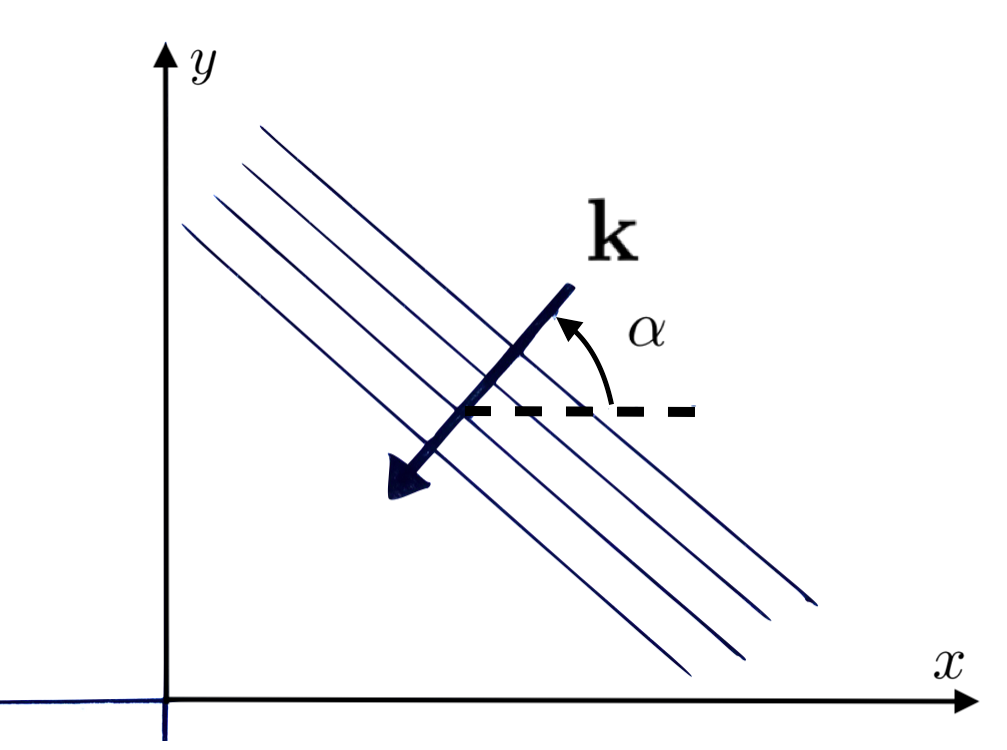
\includegraphics[width=6cm]{derivation/deriv_figures/sk_incident_wave_2.png}
        \caption{Incident wave with wave vector $\vec{k}$}
        \label{fig:incident_wave}
    \end{figure}
%
We can interpret the constants we have stated in this chapter physically.\par
%
    \begin{defn}\label{defn:wave_vector}
    The \emph{wave vector} $\vec{k}$ of a 2D plane wave is defined as
        \[ \vec{k} = (a, b) = -(k\cos\alpha, k\sin\alpha)
        \]
    where $k$ is the \emph{wave number} and $\alpha$ is the \emph{incident angle} of the wave as shown in \figref{fig:incident_wave}. 
    \end{defn}\par
%
Physically, the wave number corresponds to the number of oscillations per unit distance, and is inversely proportional to the wavelength $\lambda$:\par
    \begin{equation}
        k = \frac{2\pi}{\lambda}.
    \end{equation}\par
%
In \ssref{ss:time_dependece} we defined $\omega=kc$, where $c$ is the speed of sound. This has a physical interpretation.
    \begin{defn}
    The frequency of a plane wave with wave vector $\vec{k}$ is $kc= \omega$.
    \end{defn}\par
%
In the following chapters, we will be concerned with finding expressions for the velocity fields of a plane wave scattered by some object. \par
%
In \ssref{ss:lin_wave_eq} we showed that $\vec{u}=\nabla\phi$, and that this function $\phi$ satisfies the linear wave equation. Additionally, we found a general expression for the time dependency of $\phi$, and we showed that its spatial dependency is determined by the Helmholtz equation \eqref{eq:helmholtz}. \par
%
    \begin{propn} \label{prop:ch1_small_phi_defn}
    We can express $\phi$ as follows
        \begin{equation}\label{eq:phi_to_complex}
            \phi(x,y,z,t) = \Re[ \Phi(x,y,z)e^{-i\omega t} ].
        \end{equation}
    \end{propn}
    \begin{proof}
    Let $\Phi=\Phi_r+i\Phi_i$. Then,
        \begin{align*} 
        \Phi e^{-i\omega t} 
        &= (\Phi_r+i\Phi_i) (\cos(\omega t) - i\sin(\omega t)) \\
        &= \Phi_r \cos(\omega t) 
            - i \Phi_r \sin(\omega t)
            + i \Phi_i \cos(\omega t) 
            - (i)^2 \Phi_i \sin(\omega t)\\
        \therefore~ \Re[\Phi e^{-i\omega t}]
        &= \Phi_r \cos(\omega t) + \Phi_i \sin(\omega t)
        \end{align*}
    Clearly this would work just as well for $e^{i \omega t}$, we would just need a different choice of $\Phi_i.$\par
    %
    Clearly, \eqref{eq:phi_to_complex} is a solution to the time dependent differential equation \eqref{eq:helmholtz_time_dep}, since $\Phi_{r, i}$ do not depend on $t$. \par
    %
    We also require that $\phi$ satisfy the Linear Wave Equation \eqref{eq:lin_wave_phi}. Then,
        \begin{align*}
            \nabla^2 \phi &= \frac{1}{c^2} \partialfrac{^2 \phi}{t} \\
            \Re[ \nabla^2 \Phi(x,y,z)e^{-i\omega t} ]
            &= \Re \left[ \frac{1}{c^2} \partialfrac{^2 }{t} (\Phi(x,y,z)e^{-i\omega t}) \right]
        \end{align*}
        \begin{align*}
            \Re \left[
            \nabla^2 \Phi e^{-i\omega t} 
            - \frac{1}{c^2}(-\omega^2) \Phi e^{-i\omega t}
            \right] &= 0 \\
            \Re \left[
            e^{-i\omega t} (\nabla^2\Phi + k^2\Phi)
            \right] &= 0.
        \end{align*}
    Since this must hold for all $t$,
        \begin{equation*}
            \nabla^2 \Phi +k^2 \Phi = 0
        \end{equation*}
    as required. 
    \end{proof}